\noindent In vielen praktischen Anwendungen werden analoge Signale mit digitalen Systemen wie zum Beispiel Computern oder Mikro-Controllern erfasst und digital verarbeitet. Gründe für die digitale Realisierung von Systemen sind die kostengünstige Umsetzung, die sich aus der Verwendung von Mikro-Controllern oder hochintegrierter Schaltungen ergibt, und die Anwendung von Algorithmen, die analog wenn überhaupt nur sehr aufwendig umgesetzt werden können. 

\noindent Der Aufbau eines Systems zur digitalen Signalverarbeitung ist in Bild \ref{fig:SignalflussDSV} dargestellt. Bei der Beschreibung eines Abtastvorgangs wird sich zeigen, dass das abzutastende Signal zunächst durch einen Tiefpass bandbegrenzt werden muss. Nach der anschlie{\ss}enden Abtastung liegen zeitdiskrete Signalwerte vor, mit den eine digitale Signalverarbeitung (DSV) durchgeführt wird. Gegebenenfalls werden die zeitdiskreten Abtastwerte über ein Halteglied und einen Tiefpass zu einem analogen Signal rekonstruiert. Insgesamt ergibt sich damit die in Bild \ref{fig:SignalflussDSV} beschriebene Signalverarbeitungskette.


\begin{figure}[H]
  \centerline{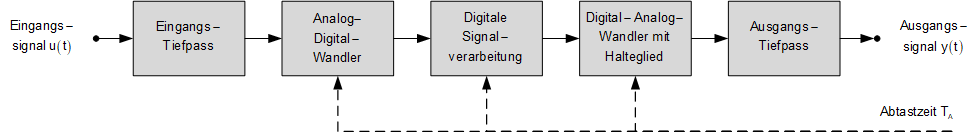
\includegraphics[width=1\textwidth]{Einleitung/Bilder/image1.png}}
  \caption{Blockdiagramm zur digitalen Signalverarbeitung}
  \label{fig:SignalflussDSV}
\end{figure}

\noindent Die Signalverarbeitung wird dabei in Form von Gleichungen oder Algorithmen beschrieben, die von digitalen Systemen in einfacher Form umgesetzt werden können. Au{\ss}er einer Speicherverwaltung müssen zur Realisierung der Algorithmen über Differenzengleichung nur Multiplikation und Additionen durchgeführt werden. Damit können die Algorithmen in sehr unterschiedlichen Systemen implementiert werden. Bei Anwendungen mit hohen Stückzahlen wie im Automotive-Bereich und bei Smart-Phones werden Application-Specific-Integrated-Circuits (ASIC) mit digitaler Signalverarbeitung eingesetzt. Zur Steuerung von Prozessen und zur lokalen Signalverarbeitung werden Mikro-Controller und digitale Signalprozessoren sowie Field-Programmable-Gate-Arrays (FPGA) eingesetzt. Auch in der Automatisierungstechnik findet die digitale Signalverarbeitung Anwendung. Bild \ref{fig:BsplfürSystememitdigitalerSignalverarbeitung} zeigt eine Auswahl von Systemen, mit denen eine digitale Signalverarbeitung realisiert wird. Der Entwurf der entsprechenden Algorithmen ist Gegenstand der folgenden Kapitel dieses Skriptes.

\clearpage

\begin{figure}[h]

\begin{subfigure}{0.5\textwidth}
\caption{Application-Specific-Integrated-Circuit (ASIC) mit digitaler Signalverarbeitung [Frit20]}
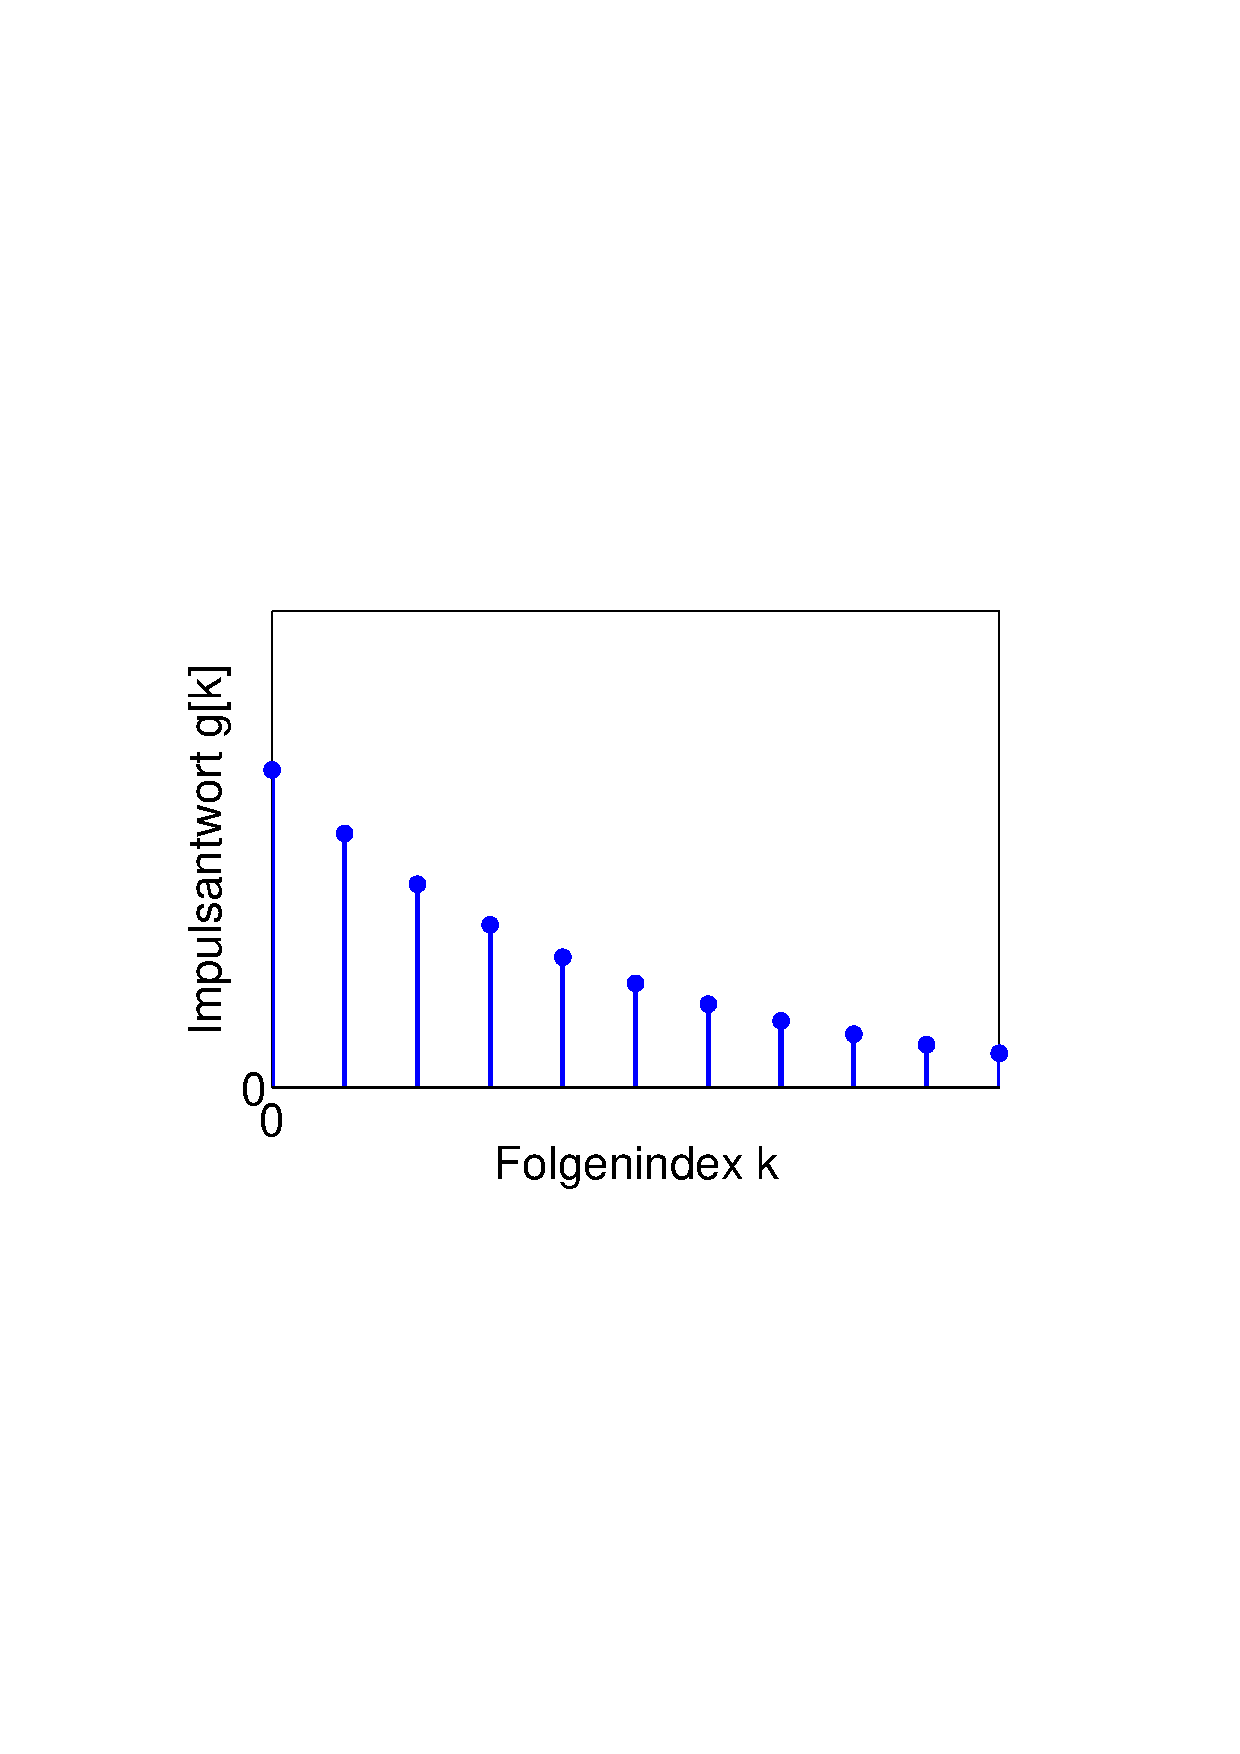
\includegraphics[width=0.9\linewidth, height=5cm]{Einleitung/Bilder/image2.jpg} 
\label{fig:subim1}
\end{subfigure}
\begin{subfigure}{0.5\textwidth}
\caption{Speicher-Programmierbare-Steuerung (SPS)}
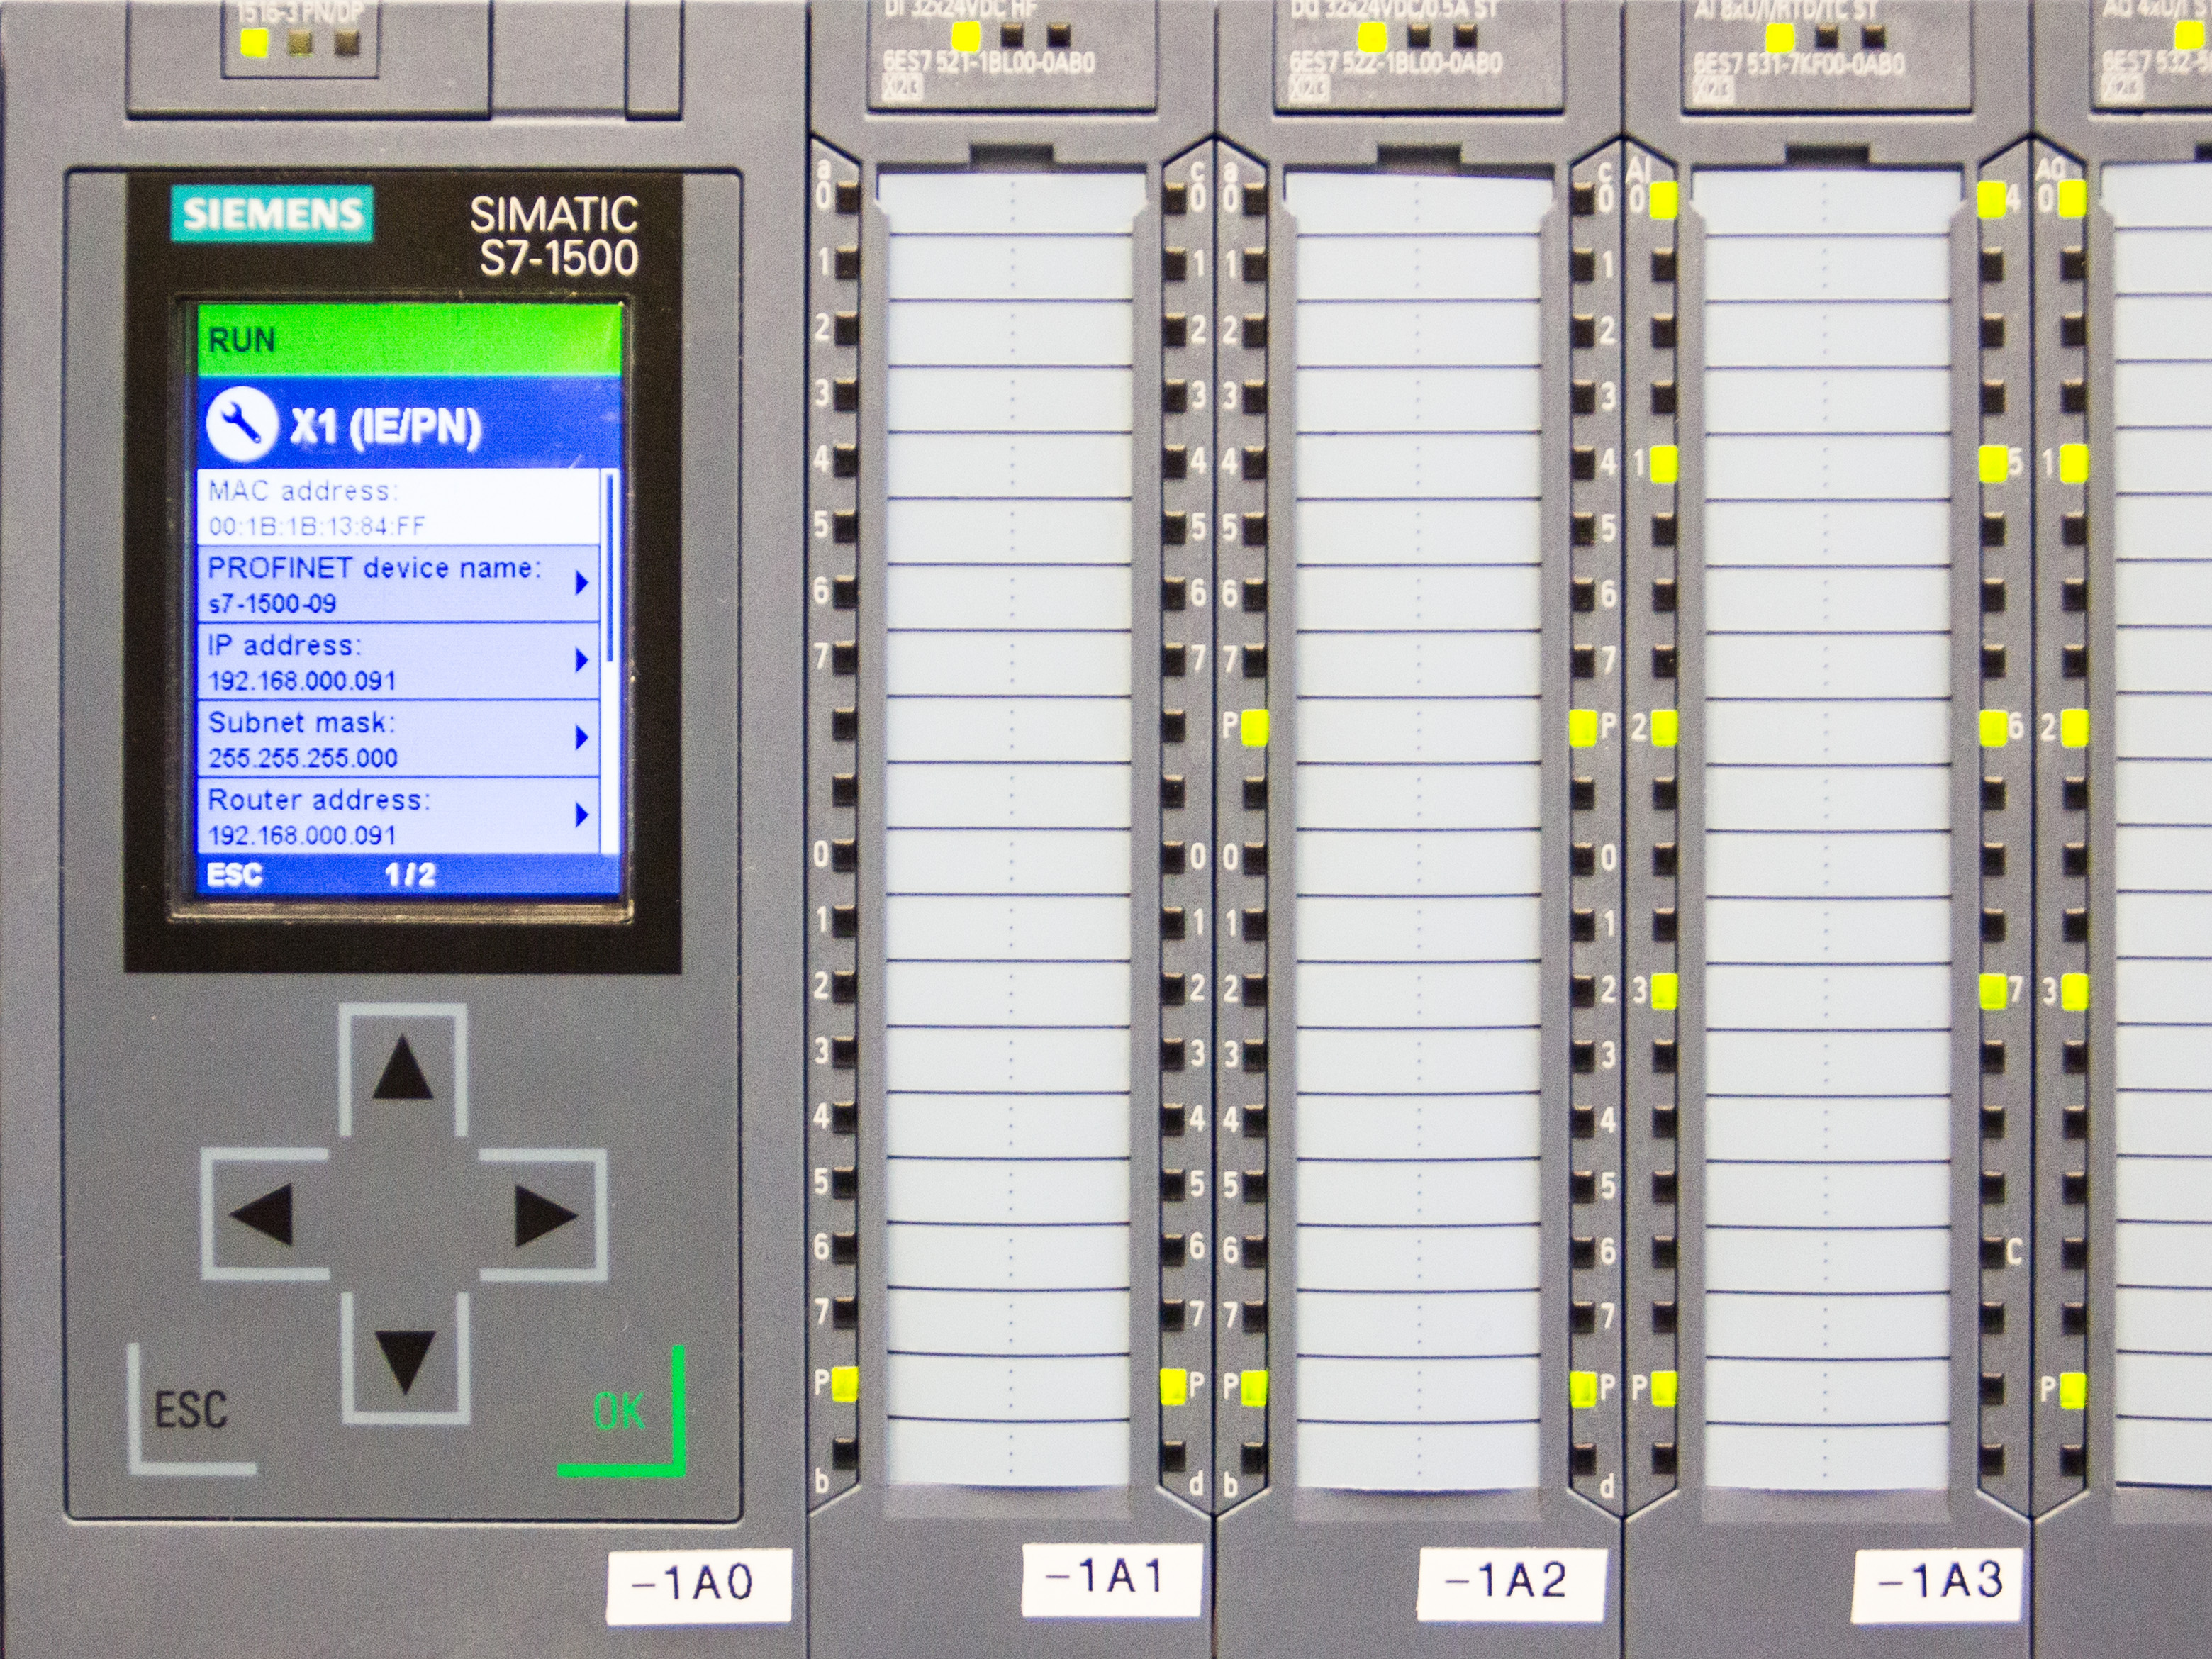
\includegraphics[width=0.9\linewidth, height=5cm]{Einleitung/Bilder/image3.jpg}
\label{fig:subim2}
\end{subfigure}
\begin{subfigure}{0.5\textwidth}
\caption{Field-Programmable-Gate-Array (FPGA)}
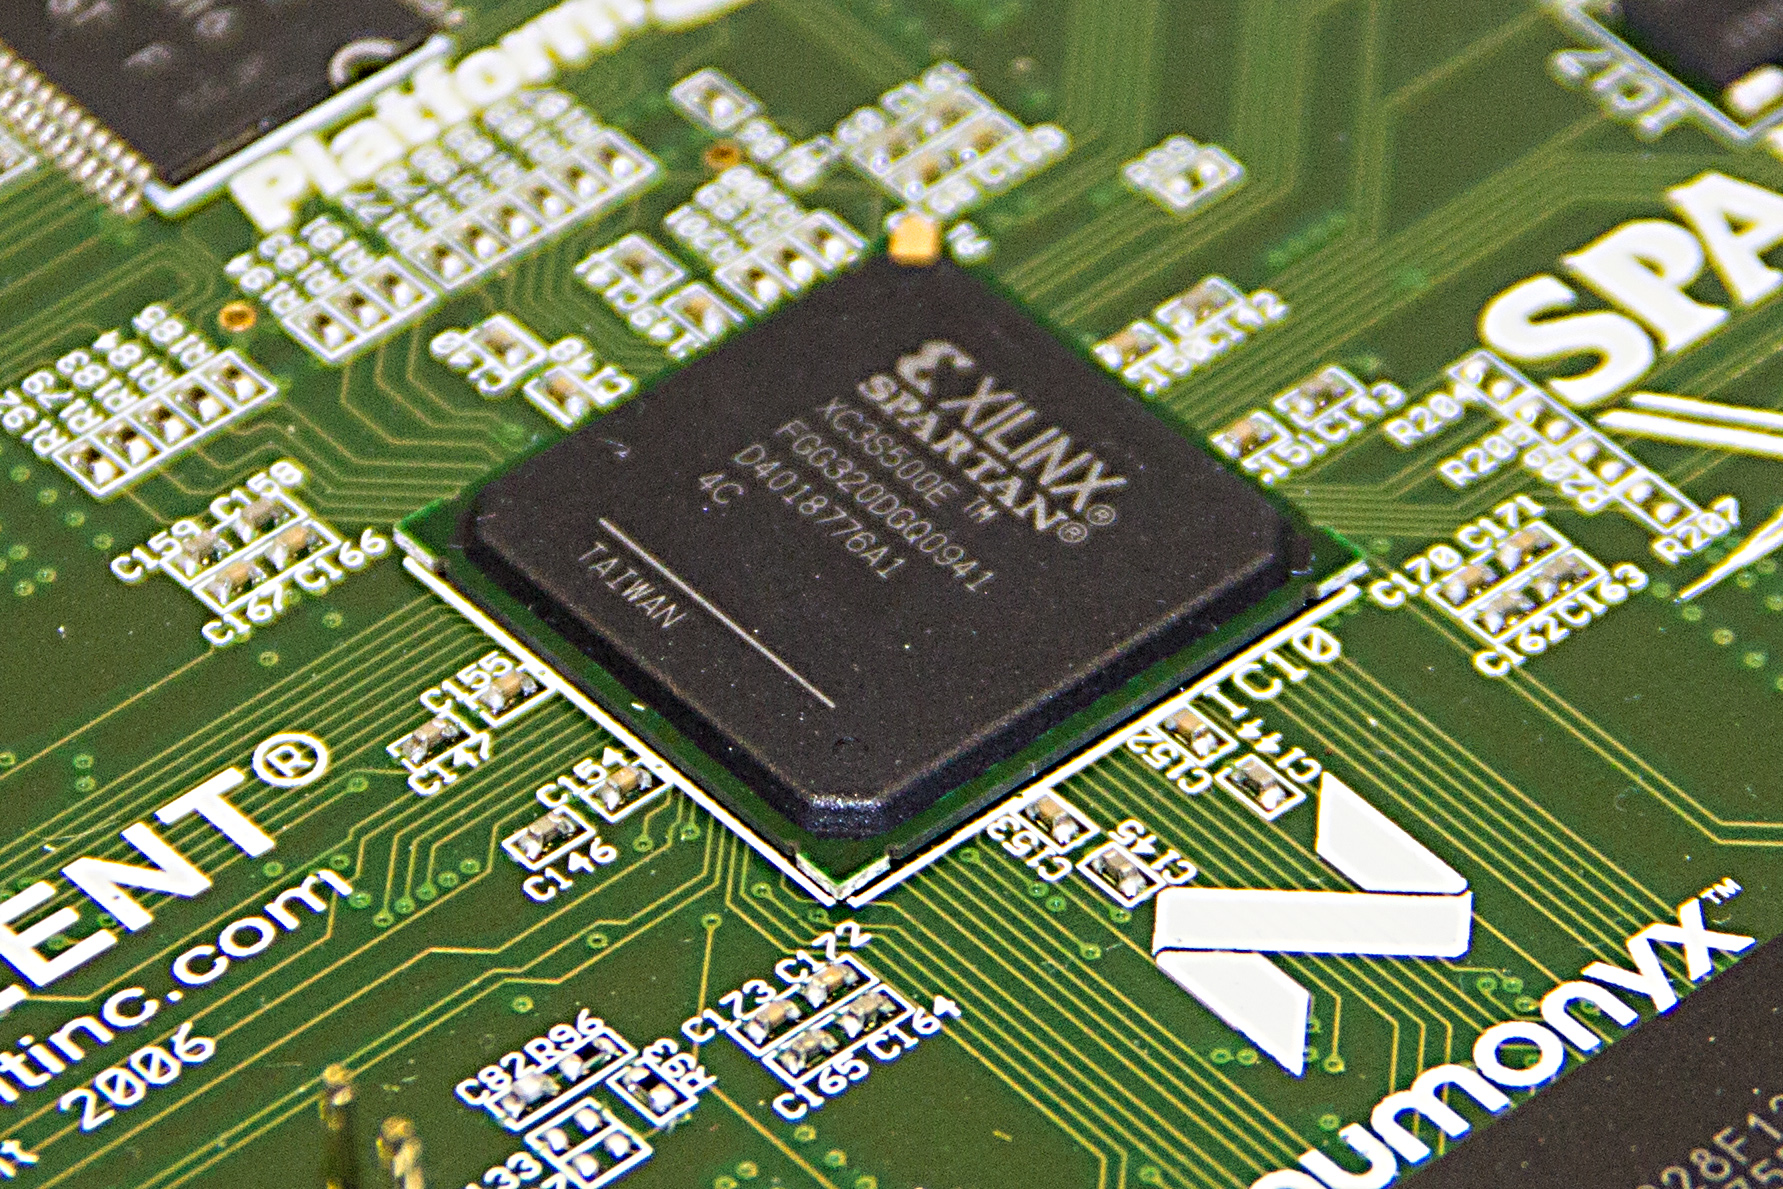
\includegraphics[width=0.9\linewidth, height=5cm]{Einleitung/Bilder/image4.jpg}
\label{fig:subim3}
\end{subfigure}
\begin{subfigure}{0.5\textwidth}
\caption{Micro-Controller (µC) und digitale Signal-prozessoren (DSP)}
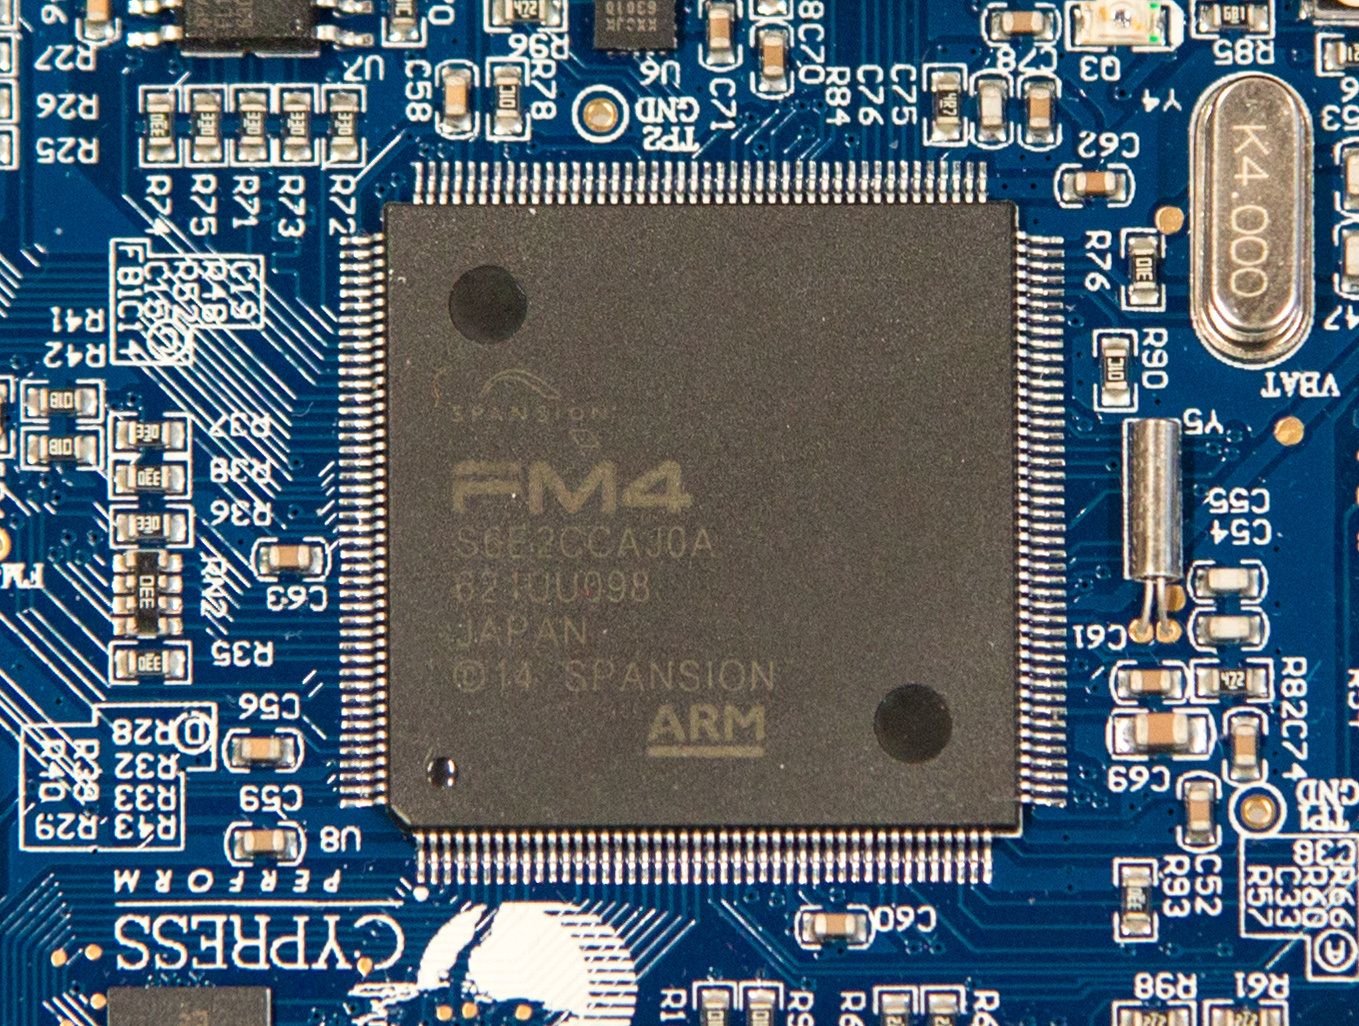
\includegraphics[width=0.9\linewidth, height=5cm]{Einleitung/Bilder/image5.jpg}
\label{fig:subim4}
\end{subfigure}
\caption{Beispiele für Systeme mit digitaler Signalverarbeitung}
\label{fig:BsplfürSystememitdigitalerSignalverarbeitung}
\end{figure}

\subsection{ Strukturierung des Buchs }

\noindent Das Buch beginnt mit der Aufgabenstellung, analoge Signale in zeitdiskrete Signale umzusetzen. Es wird sich zeigen, dass analoge Signale ohne Verf\"{a}lschung diskretisiert werden k\"{o}nnen, wenn das sogenannte Abtasttheorem eingehalten wird. Kritischer ist eine technisch realisierbare Rekonstruktion der Abtastwerte zu einem zeitkontinuierlichen Signal.\medskip
\noindent Durch den Abtastprozess entstehen Zahlenfolgen. Diese Zahlen k\"{o}nnen \"{a}hnlich wie analoge Zeitfunktionen betrachtet werden. Der Umgang mit Zahlenfolgen wird dargestellt und an Beispielen ge\"{u}bt. Dabei wird das Rechnen mit Impuls- und Sprungfolgen eingef\"{u}hrt und vertieft. Besonderer Wert wird auf komplexe Exponentialfolgen gelegt, die f\"{u}r das Einschwingverhalten digitaler Systeme von besonderer Bedeutung sind.\medskip

\noindent Digitale Systeme lassen sich wegen ihrer diskreten Signale nicht \"{u}ber Differentialgleichungen beschreiben. Deshalb wird die Beschreibung zeitdiskreter Systeme \"{u}ber Differenzengleichungen eingef\"{u}hrt. An Beispielen wird erl\"{a}utert, wie diese Differenzengleichungen aufgestellt werden k\"{o}nnen. Abschlie{\ss}end werden grundlegende Systemeigenschaften wie Linearit\"{a}t, Zeitinvarianz, Stabilit\"{a}t und Kausalit\"{a}t diskutiert. F\"{u}r lineare, zeitinvariante Systeme wird die Systemantwort \"{u}ber die Faltungssumme berechnet.\medskip

\noindent Die Zweiteilung von Signalen und Systemen zieht sich weiter durch das Skript. Zur L\"{o}sung von Differenzengleichungen wird die z-Transformation eingef\"{u}hrt. Sie ist das Pendant zur Laplace-Transformation zeitkontinuierlicher Signale und Systeme. Nach der Diskussion der z-Transformation f\"{u}r Signale werden Differenzengleichungen mit Hilfe der z-Transformation gel\"{o}st, und es wird der Begriff der \"{U}bertragungsfunktion zeitdiskreter Systeme eingef\"{u}hrt. An der \"{U}bertragungsfunktion k\"{o}nnen wichtige Systemeigenschaften direkt abgelesen werden, ohne die Systemantwort ausrechnen zu m\"{u}ssen. Die Interpretation der \"{U}bertragungsfunktion wird beschrieben und an Beispielen angewendet.\medskip

\noindent Anschlie{\ss}end wird der Begriff des Spektrums einer Signalfolge erl\"{a}utert, und es wird die Fourier-Transformation von Signalfolgen vorgestellt. Mit der Fourier-Transformation f\"{u}r Signalfolgen wird einer Signalfolge ein Spektrum zugeordnet. Zeitdiskrete Systeme weisen einen Frequenzgang auf, der ebenfalls \"{u}ber die Fourier-Transformation von Signalfolgen bestimmt werden kann. Durchlaufen zeitdiskrete Signale zeitdiskrete Systeme, wird ihr Spektrum mit dem Frequenzgang des Systems multipliziert.\medskip

\noindent In Produkten werden zeitkontinuierliche Systeme als Ersatz oder Erg\"{a}nzung zu zeitdiskreten Systemen eingesetzt. Dabei wird sich eine zeitdiskrete Realisierung im Detail immer von einer zeitkontinuierlichen Realisierung unterscheiden. Es stellt sich die Frage, wie ein zeitkontinuierliches System vorteilhaft zeitdiskret approximiert werden kann.\medskip

\noindent F\"{u}r eine gezielte \"{A}nderung des Spektrums k\"{o}nnen zeitdiskrete Filter entworfen werden. Dazu werden unterschiedliche Verfahren zum Filter-Design f\"{u}r Filter mit endlicher Impulsantwort (FIR-Filter) und f\"{u}r Filter mit unendlicher Impulsantwort (IIR-Filter) beschrieben und an Beispielen verdeutlicht. F\"{u}r die Realisierung von Filtern Filter werden oftmals feste Strukturen verwendet, die vergleichbar zu standardisierten Operationsverst\"{a}rkerschaltungen f\"{u}r analoge Filter sind. \medskip

\noindent Zur Bestimmung des Spektrums eines gemessenen Signals wird die Diskrete-Fourier-Transformation verwendet. Sie wird am Ende des Skriptes vorgestellt und angewendet. Durch eine Analyse des Signalflusses von der zeitkontinuierlichen Funktion bis zum Spektrum der Diskreten-Fourier Transformation werden Effekte wie Leakage, Zero-Padding und Fensterung erl\"{a}utert.\medskip

\noindent Die Darstellungen in diesem Skript werden mit Beispielen illustriert. Beispiele beginnen mit einem grauen Balken und enden mit einem kleinen Quadrat.\bigskip

\noindent
\colorbox{lightgray}{%
\arrayrulecolor{white}%
\renewcommand\arraystretch{0.6}%
\begin{tabular}{ wl{16.5cm} }
{\fontfamily{phv}\selectfont
\noindent{Beispiel:  }}
\end{tabular}%
}\medskip

\noindent Erläuterung des Beispiels \medskip

\noindent Wesentlicher Erfolgsfaktor f\"{u}r das Verst\"{a}ndnis und den praktischen Umgang mit den Methoden der Systemtheorie ist das selbstst\"{a}ndige Rechnen von Aufgaben. Aus diesem Grund sind in das vorliegende Buch \"{U}bungsaufgaben integriert, die eine Semester begleitende Vertiefung erm\"{o}glichen. Musterl\"{o}sungen sind online verf\"{u}gbar.

\clearpage


\subsection{Ergänzungen zum Buch}

\noindent Das Fach Systemtheorie f\"{u}hrt zu interdisziplin\"{a}ren Systembeschreibungen und bietet damit die Option, unterschiedliche Disziplinen und Fachrichtungen miteinander zu verbinden. Dies ist vor allem bei gr\"{o}{\ss}eren Entwicklungsprojekten in Industrie und Wirtschaft von strategischer Bedeutung. Leider steht der hohen Bedeutung oft eine Abneigung der Studierenden gegen\"{u}ber, die das Fach Systemtheorie als theoretisch und abstrakt empfinden. In einem Projekt Systemtheorie-Online, das von der Hochschule Karlsruhe und dem Land Baden-W\"{u}rttemberg gef\"{o}rdert wurde, wurden unterschiedliche Elemente entwickelt, mit denen die Praxisrelevanz des Stoffes verdeutlicht und die Motivation der Studierenden gesteigert werden soll. 


\subsubsection{Systemtheorie-Online}

\noindent Eine Ma{\ss}nahme ist die Online-Plattform Systemtheorie-Online. Bei der Online-Plattform handelt es sich um ein Internet-Portal zur Unterstützung des Vorlesungsbetriebs. Die Studierenden haben dort die Möglichkeit, das Skript als PDF-Dokument herunterzuladen oder es online mit mehreren Zusatzfunktionen durchzuarbeiten. Zu den präsentierten Inhalten werden themenbezogen Links zu Praxisbeispielen und Übungsaufgaben sowie sogenannte Applikationen und sogenannte virtuelle Versuche bereitgestellt.


\begin{figure}[H]
  \centerline{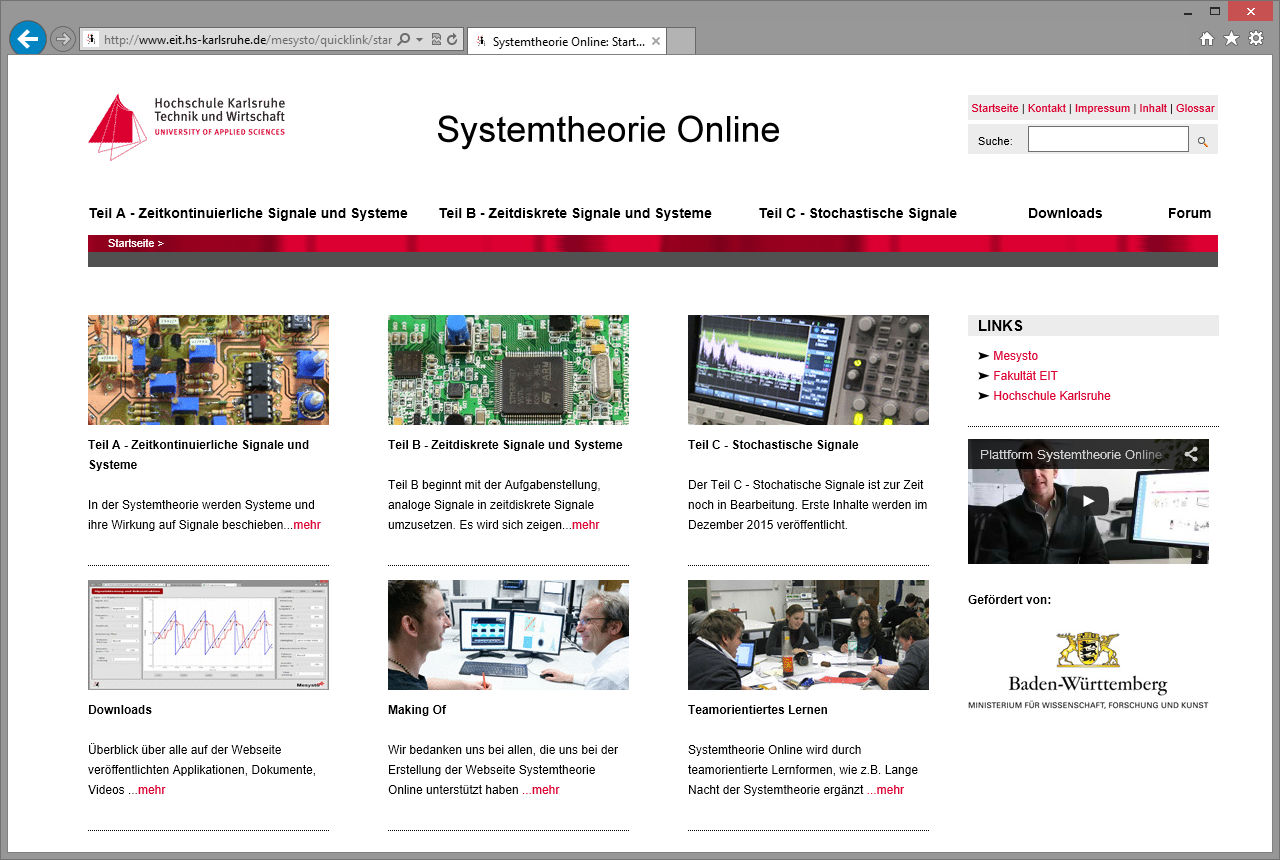
\includegraphics[width=0.6\textwidth]{Einleitung/Bilder/image6.png}}
  \caption{Systemtheorie Online (www.hs-karlsruhe.de/mesysto)}
  \label{fig:SySOnline}
\end{figure}

\medskip

{\fontfamily{phv}\selectfont
\noindent\textbf{Applikationen zur Systemtheorie}} \smallskip

\noindent Für Sachverhalte und Zusammenhänge, die sich die Studierenden nur schwer vorstellen können, werden Applikationen zur Verfügung gestellt. Bei den Applikationen können Parameter beispielsweise per Schiebregler verändert und die Folgen dieser Modifikationen auf die Ausgabesignale beobachtet werden. Die Applikationen erlauben es einerseits, im Rahmen des spielerischen Ausprobierens ein Gefühl für Zusammenhänge und Abhängigkeiten verschiedener Systemparameter zu bekommen. In Video-Tutorials werden Studierenden in den Umgang mit den Applikationen eingeführt. Sie sollen dabei vor der Manipulation von Parametern Hypothesen über zu erwartende Effekte auf das Gesamtsystem abgeben, bevor unmittelbar darauf das Ergebnis-Feedback bezüglich des Zutreffens des eigenen Vorhersagen erfolgt. 

\clearpage

\noindent Das Vorgehen bei den grafischen Animationen kann kurz an einem Beispiel erläutert werden: Ein PT2-Glied ist von den Parametern Zeitkonstante T, Dämpfung d und Verstärkung k abhängig (Bild \ref{fig:PT2-Gliede}). Die grafische Animation zeigt parallel die Eigenschaften des Systems im Zeit-, Laplace- und Frequenzbereich. Die Parameter können dabei durch Schieberegler variiert werden, sodass die Studierenden spielend ein Fingerspitzengefühl für das Übertragungsverhalten bekommen. Durch die Bereitstellung als Silverlight-Applikation benötigen die Studierenden keine zusätzliche Software, um das Programm auszuführen.

\begin{figure}[H]
  \centerline{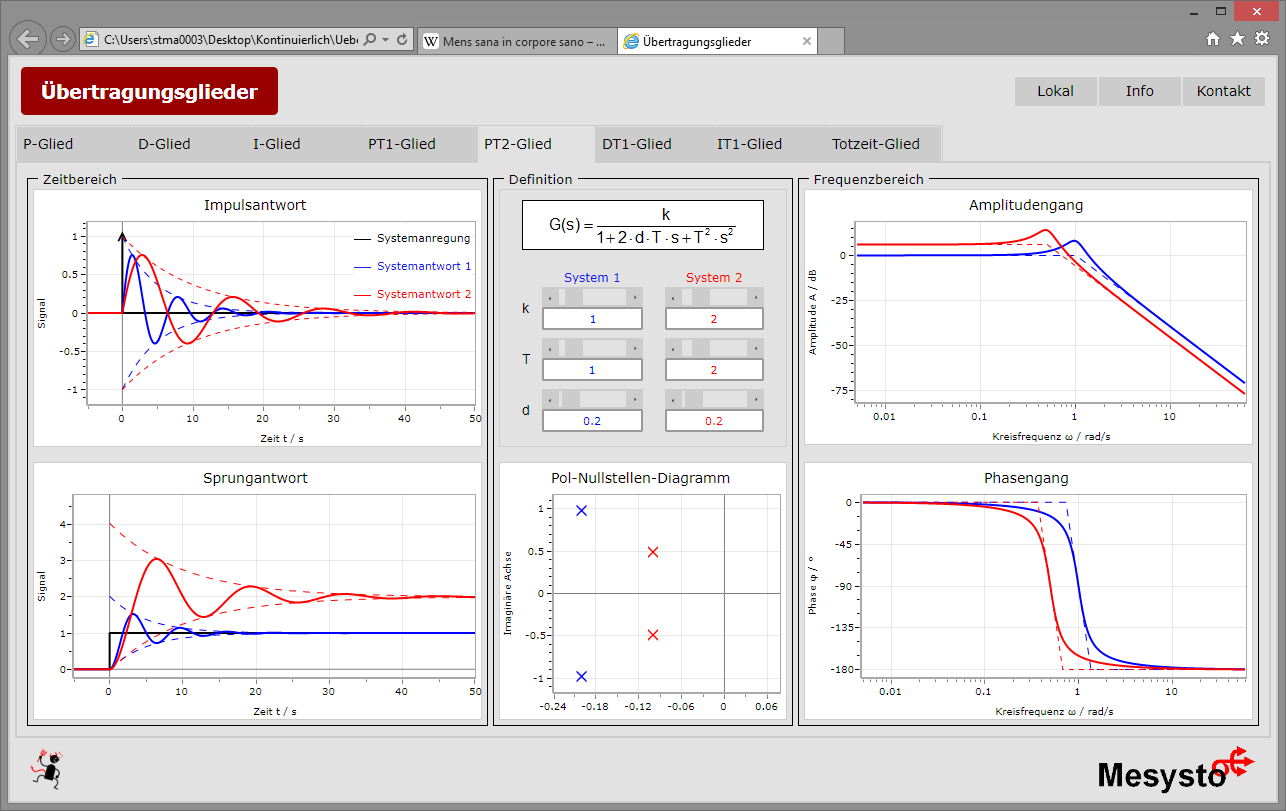
\includegraphics[width=0.6\textwidth]{Einleitung/Bilder/image7.png}}
  \caption{Darstellung des Verhaltens eines sogenannten PT2-Gliedes als Silverlight-Applikation}
  \label{fig:PT2-Gliede}
\end{figure}
\medskip

{\fontfamily{phv}\selectfont
\noindent\textbf{Virtuelle Versuche zur Systemtheorie}} \smallskip

\noindent Darüber ermöglicht die Online-Plattform die Durchführung virtueller Experimente. Passend zu den Themen des Skripts werden Versuche mit dem Laborwagen auf Video aufgezeichnet und diese auf der Online-Plattform gemeinsam mit den entsprechenden Datensätzen zur Verfügung gestellt. Zusätzliche Erläuterungen zur Durchführung der Versuche und Auswertung der Daten fördern ein Grundverständnis für das wissenschaftliche Denken und Arbeiten. 

\noindent Als Experimente zur Demonstration stehen bereits einige Versuche zum Laborwagen zur Verfügung. Bild \ref{fig:Lautsprecher} zeigt zum Beispiel einen Versuch zur Beschreibung des Einschwingverhaltens eines Lautsprechers. Weitere Experimente insbesondere zu den Themen diskrete Systeme und stochastische Systeme wurden aufgebaut und gefilmt, die Videos stehen als Datei zur Verfügung. Die Studierenden erhalten aber nicht nur den Video-Stream, sondern auch die einzelnen Versuchsergebnisse in Form von Daten-Files und können bei Interesse eigene Versuchsauswertungen erstellen. 
\clearpage

\begin{figure}[H]
  \centerline{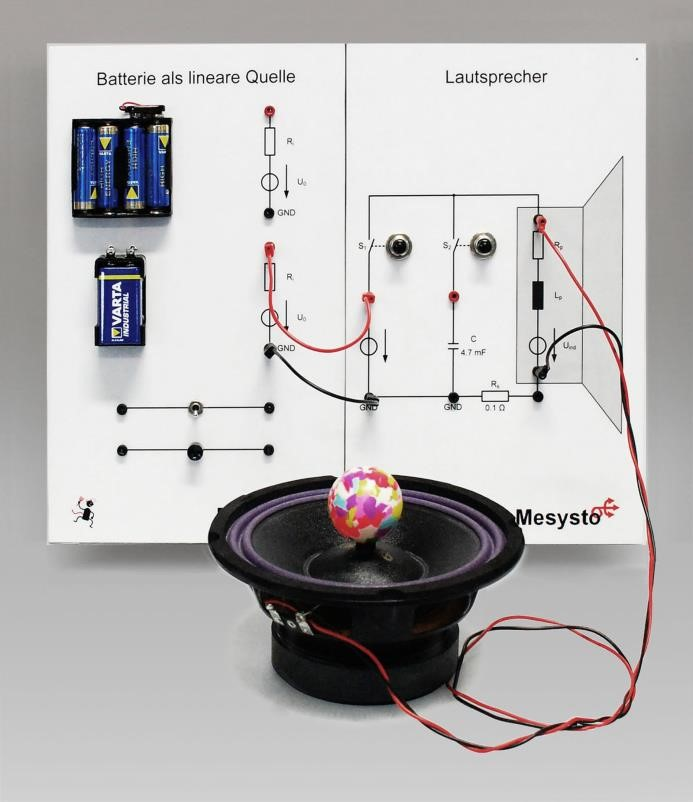
\includegraphics[width=0.55\textwidth]{Einleitung/Bilder/image8.jpg}}
  \caption{Versuchsaufbau zum Einschwingverhalten eines Lautsprechers}
  \label{fig:Lautsprecher}
\end{figure}


\noindent Das Portal Systemtheorie-Online bietet den Studierenden damit die Möglichkeit, theoretische Sachverhalte auf eine anschauliche Art aufbereitet und erklärt zu bekommen. Damit wird eine Forderung aus der Evaluation aufgegriffen, mehr Versuche in der Systemtheorie einzusetzen. Darüber hinaus haben die Studierenden die Möglichkeit, selbst aktiv zu werden und Versuche selbstständig auszuwerten und daran ihren eigenen Lernerfolg zu messen. Das Projekt bietet damit einen Beitrag zur praxisnahen Ausbildung von Studierenden und stellt wegen des freien Zugangs ein Weiterbildungsangebot dar, das Mitarbeitern aus Industrie und Wirtschaft offensteht. Der Aufbau dieses Portal wurde im Rahmen von Pro-Studium aus Studiengebühren und aus Mitteln des Landes Baden-Württemberg im Rahmen des Programms Willkommen in der Wissenschaft finanziert.


\subsubsection{Teamorientierte Lehrmethoden}

\noindent Parallel zu den Online-Aktivitäten wird die Vorlesung um unterschiedliche teamorientierte Lehrmethoden erg\"{a}nzt. Kooperative Lernformen f\"{o}rdern den Zusammenhalt und tragen sozialen Bed\"{u}rfnissen Rechnung. Sie wirken der sozialen Isolation entgegen, die Studierenden f\"{u}hlen sich eingebunden. Nicht zuletzt spiegelt die Teamarbeit auch berufliche Anforderungen wider. Die Methoden des teamorientierten Lernens sind auf der Online-Plattform ausf\"{u}hrlich dokumentiert.\bigskip

{\fontfamily{phv}\selectfont
\noindent\textbf{Lange Nächte der Systemtheorie}} \smallskip

\noindent Lange N\"{a}chte sind abendliche Veranstaltungen zur Vertiefung des Vorlesungsstoffs, passend zu einem bestimmten Vorlesungsthema. In entspannter Atmosph\"{a}re werden \"{U}bungsaufgaben und Experimente mit dem Laborwagen miteinander kombiniert. Der verf\"{u}gbare Zeitrahmen erlaubt eine Besch\"{a}ftigung mit komplexeren Fragestellungen. In erster Linie ist dieser Baustein als offener Lernraum konzipiert, in dem Wissen stressfrei vermittelt und vertieft wird. Erste lange N\"{a}chte wurden von den Studierenden sehr positiv bewertet. Besonders gelobt wurden das gemeinschaftliche Lernen in der Gruppe, das angenehme Arbeitsklima sowie der Praxisbezug und die Arbeit mit realen Messdaten.

\clearpage

{\fontfamily{phv}\selectfont
\noindent\textbf{Gro{\ss}er Preis der Systemtheorie}} \smallskip

\noindent In Anlehnung an die Fernsehsendung "Der gro{\ss}e Preis" wird mit den Studierenden eine Quiz-Show veranstaltet. Dabei bearbeiten die Studierenden in Gruppen Fragen zu Themenbl\"{o}cken der Vorlesung. Die Punktzahl ist abh\"{a}ngig von Schwierigkeitsgrad. Die Absch\"{a}tzung eines Einsatzes bei sogenannten Risiko-Fragen erfordert die Selbsteinsch\"{a}tzung der Studierenden. Durch sogenannte Gl\"{u}cksfragen zu fachfremden Themen k\"{o}nnen auch Gruppen mit m\"{a}{\ss}igem Fachwissen gewinnen. Die traditionelle Rangordnung innerhalb der Vorlesung wird aufgebrochen und die Motivation der Studierenden steigt. Studierenden zeigten bei erster Durchf\"{u}hrung extrem hohe Motivation und hohes Engagement.\bigskip

{\fontfamily{phv}\selectfont
\noindent\textbf{Zirkeltraining Systemtheorie}} \smallskip

\noindent Erfolgreiches Lernen setzt ein Gleichgewicht zwischen Anspannung und Entspannung voraus. Zielsetzung dieses Zirkeltrainings ist es deshalb, sportliche \"{U}bungen oder Geschicklichkeitsspiele in den Lernprozess zu integrieren. Dazu wird ein Parkour aufgebaut, bei dem sich \"{U}bungsaufgaben und Spielstationen abwechseln. Bei der Veranstaltung stehen die Motivation und der Spa{\ss} an vorderster Stelle. Es wird eine angenehme Atmosph\"{a}re geschaffen, in der der Druck beim Bew\"{a}ltigen von \"{U}bungsaufgaben durch spielerische Anteile entlastet wird. Wegen des erforderlichen Platzbedarfs eignet sich das Zirkeltraining Systemtheorie insbesondere f\"{u}r die Sommermonate.

\noindent Die Evaluationsergebnisse zur Vorlesung zeigen, dass es durch den Einsatz teamorientierter Lehrmethoden gelungen ist, diese Abneigung gegen das Fach Systemtheorie zumindest teilweise abzubauen. 

\clearpage


\subsection{Danksagung}

\noindent Wir bedanken uns bei den Studierenden und Assistenten Andreas K\"{u}hn, Erik Seiter, Sebastian Stiegler, Philipp Fetzer, Jaruwan Limsukhakorn, Doraemon Dedkum, Georg Bauer, Jochen Lang, Alex Schwin und Michael Holz f\"{u}r die Gestaltung und Ausarbeitung des wesentlichen Teils der \"{U}bungsaufgaben, Applikationen und Versuche.

\noindent Unserer besonderer Dank gilt au{\ss}erdem den Kollegen Prof. Dr. Beucher, Prof. Dr. Dussel, Prof. Dr. Quint und Prof. Dr. Weizenecker, die die inhaltliche und mathematische Darstellung in diesem Buch kritisch hinterfragt und damit zur besseren Verst\"{a}ndlichkeit beigetragen haben. 

\noindent In das Buch sind viele Hinweise von Studierenden der Hochschule Karlsruhe eingegangen. Wir haben versucht, den Hinweisen gerecht zu werden, die meisten Hinweise sind bereits in \"{U}berarbeitungen Korrekturen eingeflossen. \"{U}ber weitere Hinweise zur mangelhaften Verst\"{a}ndlichkeit und auf Fehler w\"{u}rden wir uns freuen. \bigskip

\noindent Karlsruhe, 16.03.2015 \bigskip

\bigskip

\bigskip

\noindent Quelle 

\begin{itemize}
    \item 35465715536\_0df591f741\_4k.jpg,  US\_IV+\_\_\_DSC00496, https://www.flickr.com/photos/130561288@N04/, Fritzchens Fritz, https://flic.kr/p/W2Z4C5, auf Flickr, CC0 1.0 Universal (CC0 1.0) Public Domain Dedication 
\end{itemize}